% =====================================================================
%  Avaliacao de danos em edificacoes a partir de imagens de satelite:
%  um estudo de ablacao distribuido sobre o xBD
%
%  Compilar:  pdflatex relatorio.tex   (duas vezes, por causa das referencias)
%
%  A foto do laboratorio e opcional: se `figuras/laboratorio.jpg` nao existir,
%  um quadro de marcacao aparece no lugar e o documento compila do mesmo jeito.
% =====================================================================
\documentclass[11pt,a4paper]{article}

\usepackage[utf8]{inputenc}
\usepackage[T1]{fontenc}
\usepackage[brazil]{babel}
\usepackage{lmodern}
\usepackage{microtype}

\usepackage{amsmath,amssymb}
\usepackage{booktabs}
\usepackage{graphicx}
\usepackage{caption}
\usepackage{subcaption}
\usepackage{xcolor}
\usepackage[margin=2.5cm]{geometry}
\usepackage{tikz}
\usepackage{pgfplots}
\pgfplotsset{compat=1.17}
\usetikzlibrary{positioning,arrows.meta,fit,backgrounds,calc,shapes.geometric}
\usepackage[hidelinks]{hyperref}

% ---- cores do documento ----
\definecolor{azul}{RGB}{31,86,158}
\definecolor{verde}{RGB}{34,120,60}
\definecolor{vermelho}{RGB}{176,42,42}
\definecolor{cinza}{RGB}{110,110,110}
\definecolor{cinzaclaro}{RGB}{235,238,242}

% ---- estilos reutilizados nos diagramas ----
\tikzset{
  bloco/.style   = {draw=azul!70, fill=azul!8, rounded corners=2pt,
                    minimum height=8mm, minimum width=18mm, font=\small,
                    align=center, inner sep=3pt},
  blocoA/.style  = {draw=verde!70, fill=verde!8, rounded corners=2pt,
                    minimum height=8mm, minimum width=18mm, font=\small,
                    align=center, inner sep=3pt},
  img/.style     = {draw=cinza, fill=cinzaclaro, minimum height=9mm,
                    minimum width=13mm, font=\small, align=center},
  seta/.style    = {-{Latex[length=2mm]}, draw=cinza!90, thick},
  rotulo/.style  = {font=\scriptsize\itshape, text=cinza},
}

\title{\textbf{Avaliação de danos em edificações a partir de imagens\\
de satélite: um estudo de ablação distribuído sobre o xBD}}
\author{Túlio Castro\thanks{Correspondência: \texttt{tulio.castro@orbiconecta.com.br}.
Código, dados derivados e documentação completa em
\texttt{github.com/Tulio-CS/Disaster-Damage}.}}
\date{\today}

\begin{document}
\maketitle

\begin{abstract}
\noindent
Modelos de avaliação automática de danos a partir de imagens de satélite pré e
pós-desastre são tipicamente reportados no protocolo oficial do desafio xView2,
que divide as cenas de forma espacialmente correlacionada. Mostramos que esse
protocolo superestima em \textbf{32{,}3\%} a capacidade real de generalização, e
que a degradação é fortemente assimétrica: a \emph{localização} de edificações
transfere quase intacta para um desastre não visto ($-3{,}1\%$), enquanto a
\emph{classificação de severidade} praticamente colapsa ($-50{,}6\%$). Para
chegar a esse resultado, executamos 24 experimentos controlados --- uma
configuração de referência, oito \emph{baselines} e quinze ablações de um fator
--- em 10 estações de trabalho com GPU coordenadas por uma fila central, em um
único dia de laboratório. Três réplicas de semente estabelecem um piso de ruído
de $0{,}0068$, contra o qual todo efeito é julgado. Entre os achados: o termo de
diferença explícita em espaço de \emph{features}, premissa do desenho
arquitetural, não se paga; capacidade de modelo não é o gargalo (um
\emph{encoder} 8$\times$ menor empata com o maior); e o limitante da métrica é a
\emph{precisão} da classe \texttt{minor-damage}, não o \emph{recall}, o que
inverte a correção usualmente aplicada a desbalanceamento de classes.
\end{abstract}

\vspace{0.5em}
\noindent\textbf{Palavras-chave:} detecção de mudança, sensoriamento remoto,
segmentação semântica, redes siamesas, estudo de ablação, xBD/xView2.

\section{Introdução}

Após um desastre natural, a alocação de equipes de resgate depende de saber
\emph{onde} há edificações atingidas e \emph{quão} graves são os danos. Fazer
esse levantamento manualmente, a partir de imagens de satélite, leva dias ---
tempo que a resposta emergencial não tem. O dataset xBD~\cite{gupta2019} e o
desafio xView2~\cite{xview2} formalizaram a tarefa: dado um par de imagens
co-registradas da mesma cena, antes e depois do evento, produzir uma segmentação
em cinco classes por pixel (fundo e quatro níveis ordinais de severidade).

A prática estabelecida reporta desempenho no \emph{split} oficial do desafio.
Este trabalho parte de uma observação feita durante a análise exploratória dos
dados: em 8 dos 10 eventos avaliados, mais de dois terços dos \emph{tiles} do
conjunto de validação são espacialmente adjacentes (menos de 500\,m) a um
\emph{tile} de treino. O protocolo oficial, portanto, mede generalização para o
quarteirão vizinho --- não para um desastre novo, que é o caso de uso real.

Nossas contribuições são:

\begin{enumerate}
  \item \textbf{Quantificação do viés do protocolo oficial.} Comparando o
  \emph{split} oficial com uma validação cruzada agrupada por evento, medimos
  uma queda de 32{,}3\% no escore, decomposta em $-3{,}1\%$ na localização e
  $-50{,}6\%$ na classificação de severidade (Seção~\ref{sec:generalizacao}).

  \item \textbf{Um estudo de ablação controlado} com 24 configurações,
  disciplinado por um piso de ruído medido em réplicas de semente
  (Seção~\ref{sec:ablacoes}), incluindo três resultados negativos limpos sobre
  componentes usualmente assumidos como benéficos.

  \item \textbf{Uma metodologia de execução distribuída} em hardware de
  laboratório heterogêneo e sem privilégio administrativo, com fila de posse
  exclusiva e tolerância a falhas (Seção~\ref{sec:infra}).

  \item \textbf{Um diagnóstico do gargalo da métrica:} a média harmônica é
  dominada pela classe \texttt{minor-damage}, cujo limitante é a precisão e não
  o \emph{recall} --- o que inverte a correção intuitiva
  (Seção~\ref{sec:erros}).
\end{enumerate}

\section{Trabalhos relacionados}

A detecção de mudança em pares de imagens de sensoriamento remoto tem tratamento
consolidado com redes totalmente convolucionais siamesas. Daudt \emph{et
al.}~\cite{daudt2018} formalizam três variantes que são diretamente as nossas
ablações arquiteturais: fusão precoce (\emph{early fusion}), fusão por
concatenação de \emph{features} (\emph{FC-Siam-conc}) e fusão por diferença
(\emph{FC-Siam-diff}). A arquitetura siamesa de pesos compartilhados remonta a
Bromley \emph{et al.}~\cite{bromley1993}.

O esqueleto de segmentação é a U-Net~\cite{ronneberger2015}, cujas conexões de
atalho em resoluções intermediárias são essenciais quando os objetos de interesse
são pequenos --- no xBD, 71\% das edificações se enquadram no critério
\emph{small} do COCO~\cite{lin2014coco}. As soluções melhor colocadas no
xView2~\cite{xview2solutions} convergiram para U-Nets siamesas com combinação de
perdas focal~\cite{lin2017focal} e Dice~\cite{milletari2016}, escolha que
adotamos como configuração de referência precisamente para poder ablacioná-la.

Sobre avaliação, a inadequação de validação cruzada aleatória para dados com
estrutura espacial é bem documentada em ecologia e sensoriamento
remoto~\cite{roberts2017}, e a divisão agrupada por unidade espacial é a resposta
padrão. Aplicamos essa recomendação agrupando por \emph{evento de desastre}.

\section{Dados}

\subsection{Composição}

O xBD, na distribuição GeoTIFF, contém 11.034 pares pré/pós de cenas
$1024\times1024$ com resolução submétrica, e 850.736 polígonos de edificação
anotados. A Tabela~\ref{tab:dados} resume a partição.

A cobertura é deliberadamente diversa em geografia e em tipo de evento
(Figura~\ref{fig:mapa}): dezenove desastres em quatro continentes, abrangendo
terremoto e tsunami, enchente, erupção vulcânica, incêndio florestal e vento.
Essa diversidade é o que torna possível --- e necessária --- a validação
agrupada por evento discutida na Seção~\ref{sec:splits}: se todos os desastres
fossem do mesmo tipo, não haveria o que extrapolar.

\begin{figure}[htbp]
\centering
\IfFileExists{figuras/mapa_xbd.png}{%
  \includegraphics[width=\linewidth]{figuras/mapa_xbd.png}%
}{%
  \fbox{\begin{minipage}[c][42mm][c]{0.96\linewidth}
    \centering\color{cinza}\small
    \textbf{[ mapa de cobertura do xBD ]}\\[1mm]
    salve como \texttt{figuras/mapa\_xbd.png}
  \end{minipage}}%
}
\caption{Distribuição geográfica e tipológica dos eventos do xBD. A variedade de
mecanismos de destruição --- vento, água, fogo, abalo sísmico e material
vulcânico --- é justamente o que a validação agrupada por evento
(Seção~\ref{sec:splits}) submete a teste: cada \emph{fold} pede ao modelo que
generalize para um mecanismo que ele viu pouco ou não viu. Fonte: documentação
do desafio xView2~\cite{xview2}.}
\label{fig:mapa}
\end{figure}

\begin{table}[htbp]
\centering
\caption{Composição do xBD em número de cenas (pares pré/pós).}
\label{tab:dados}
\begin{tabular}{lrl}
\toprule
\textbf{Partição} & \textbf{Cenas} & \textbf{Uso neste trabalho} \\
\midrule
\texttt{tier1} & 2.799 & treino \\
\texttt{tier3} & 6.369 & treino (qualidade de anotação distinta) \\
\texttt{hold}  & 933   & validação \\
\texttt{test}  & 933   & não utilizado \\
\midrule
\textbf{Total} & \textbf{11.034} & \\
\bottomrule
\end{tabular}
\end{table}

\subsection{Propriedades que governaram o desenho}
\label{sec:eda}

Cinco medições da análise exploratória determinaram decisões concretas do
\emph{pipeline}, e são retomadas ao longo do texto pela referência a esta
seção (\ref{sec:eda}):

\begin{description}
  \item[Desbalanceamento de $\sim$10:1] a favor de \texttt{no-damage}, com
  composição que varia drasticamente entre eventos: 99{,}5\% de
  \texttt{no-damage} em \texttt{mexico-earthquake} contra 17{,}9\% em
  \texttt{hurricane-matthew}. $\rightarrow$ pesos por classe e reamostragem.

  \item[97\% dos pixels são fundo,] e 35\% das cenas não contêm nenhuma
  edificação. Entropia cruzada pura converge para ``preveja fundo''.
  $\rightarrow$ termo Dice na perda.

  \item[Objetos pequenos:] mediana de 575\,px$^2$ ($\approx 24\times24$ px).
  Na escala mais grosseira do \emph{encoder} (\emph{stride} 32) a edificação
  mediana ocupa menos de um pixel. $\rightarrow$ atalhos em \emph{stride} 2 e 4.

  \item[Intervalo temporal mediano de 304 dias] entre as aquisições pré e pós
  (5\% acima de 3{,}3 anos), com ângulo \emph{off-nadir} de 0\textdegree{} a
  44\textdegree. Boa parte da diferença visual entre as datas \emph{não é dano}:
  é estação, iluminação, ângulo e construção nova. $\rightarrow$ a diferença
  deve ser computada em espaço de \emph{features}, não de pixels; augmentações
  fotométricas aplicadas \emph{independentemente} a cada data.

  \item[Correlação espacial no \emph{split} oficial:] mais de dois terços dos
  \emph{tiles} de \texttt{hold} são adjacentes a \emph{tiles} de treino.
  $\rightarrow$ motiva a validação agrupada por evento (Seção~\ref{sec:splits}).
\end{description}

\subsection{Pré-processamento}

Os GeoTIFF são armazenados em \texttt{int16} sem compressão, mas com conteúdo de
8 bits; a conversão para PNG \texttt{uint8} é sem perda de informação e reduz o
volume de 139\,GB para 33\,GB. Como os polígonos pré e pós são geometricamente
idênticos (mesmos identificadores, deslocamento mediano de $10^{-7}$ px), uma
única máscara por cena é suficiente: a máscara de localização é
$\mathbb{1}[\text{máscara de dano} > 0]$.

O rótulo \texttt{un-classified} não é um quinto nível de severidade, e sim
ausência de julgamento do anotador; é mapeado para um índice ignorado e removido
de toda perda e de toda métrica.

\section{Método}

\subsection{Arquitetura}

O modelo é uma U-Net siamesa com \emph{encoder} compartilhado entre as duas
datas, ilustrada na Figura~\ref{fig:arquitetura}. Compartilhar pesos força as
duas imagens ao mesmo espaço de representação e reduz quase pela metade o número
de parâmetros: a rede não precisa reaprender a localizar edificações, precisa
compará-las.

\begin{figure}[htbp]
\centering
\begin{tikzpicture}[node distance=6mm and 10mm]

  \node[img] (pre)  {pré};
  \node[img, below=14mm of pre] (pos) {pós};

  \node[bloco, right=of pre, minimum height=9mm] (encA) {\emph{encoder}};
  \node[bloco, right=of pos, minimum height=9mm] (encB) {\emph{encoder}};
  \node[rotulo, right=1mm of encA.north east, anchor=south west]
       {pesos compartilhados};
  \draw[dashed, draw=azul!60] (encA.south) -- (encB.north);

  % coordenada auxiliar: `right=... of $(a)!0.5!(b)$` nao e sintaxe valida de
  % posicionamento; e preciso nomear o ponto medio antes.
  \coordinate (meio) at ($(encA.east)!0.5!(encB.east)$);
  \node[blocoA, right=13mm of meio, minimum height=16mm,
        minimum width=24mm] (fuse)
       {fusão\\[-1pt]{\scriptsize$[\,f_{\text{pré}} \mid f_{\text{pós}} \mid
        |f_{\text{pós}}-f_{\text{pré}}|\,]$}};

  \node[bloco, right=of fuse, minimum height=16mm] (dec) {\emph{decoder}\\
        {\scriptsize 256-128-64-32-16}};
  \node[bloco, right=of dec, minimum height=16mm, minimum width=20mm] (head)
       {saída\\{\scriptsize 5 classes}};

  \draw[seta] (pre) -- (encA);
  \draw[seta] (pos) -- (encB);
  \draw[seta] (encA) -- (fuse);
  \draw[seta] (encB) -- (fuse);
  \draw[seta] (fuse) -- (dec);
  \draw[seta] (dec)  -- (head);

  % atalhos multiescala
  \draw[seta, dashed, draw=verde!70]
    ($(fuse.north)+(0,1mm)$) to[out=60,in=120] ($(dec.north)+(0,1mm)$);
  \node[rotulo, above=7mm of dec] {atalhos em \emph{stride} 2 e 4};

  % derivacao da localizacao
  \node[rotulo, below=9mm of head, align=center, text width=34mm]
       {localização derivada:\\ $1-p(\text{fundo})$};
  \draw[seta, draw=vermelho!70] (head.south) -- ++(0,-6mm);

\end{tikzpicture}
\caption{U-Net siamesa. O \emph{encoder} é compartilhado entre as datas; a fusão
ocorre em cada escala, concatenando as \emph{features} das duas imagens com sua
diferença absoluta. Uma única cabeça de 5 classes serve às duas tarefas: a
localização é derivada de $1-p(\text{fundo})$, de modo que ambas as perdas
supervisionam o mesmo tensor de saída.}
\label{fig:arquitetura}
\end{figure}

\paragraph{Fusão.} Em cada escala $s$, as \emph{features} das duas datas são
combinadas por
\begin{equation}
  f_s = \phi_s\!\left(\left[\, f_s^{\text{pré}} \;\middle|\;
        f_s^{\text{pós}} \;\middle|\;
        \left| f_s^{\text{pós}} - f_s^{\text{pré}} \right| \,\right]\right),
  \label{eq:fusao}
\end{equation}
onde $\phi_s$ é uma convolução $1\times1$ seguida de normalização e não
linearidade. O terceiro termo codifica a hipótese central do desenho: o sinal de
dano reside na \emph{diferença em espaço de features}, e fornecê-la
explicitamente pouparia a rede de aprendê-la. A Seção~\ref{sec:ablacoes} testa
essa hipótese diretamente.

\paragraph{Cabeça única.} A localização não possui cabeça própria: sai de
$1 - p(\text{fundo})$. Cabeças independentes permitiriam que a rede localizasse
bem e classificasse mal sem que os gradientes se comunicassem. A
Tabela~\ref{tab:params} lista os tamanhos medidos.

\begin{table}[htbp]
\centering
\caption{Número de parâmetros por configuração (\emph{decoder} 256-128-64-32-16,
5 classes de saída).}
\label{tab:params}
\begin{tabular}{llrr}
\toprule
\textbf{Variante} & \textbf{\emph{Encoder}} & \textbf{Total} &
\textbf{\emph{Encoder}} \\
\midrule
Referência & \texttt{resnet34}~\cite{he2016}            & 25{,}50\,M & 21{,}28\,M \\
Fusão \texttt{cat} (sem $|\Delta|$) & \texttt{resnet34} & 25{,}14\,M & 21{,}28\,M \\
Fusão \texttt{diff} (só $|\Delta|$) & \texttt{resnet34} & 24{,}79\,M & 21{,}28\,M \\
Sem ramo siamês & \texttt{resnet34}                     & 24{,}44\,M & 21{,}28\,M \\
Maior capacidade & \texttt{seresnext50}~\cite{xie2017,hu2018} & 51{,}26\,M & 25{,}51\,M \\
Menor capacidade & \texttt{efficientnet\_b0}~\cite{tan2019}   &  6{,}19\,M &  3{,}60\,M \\
\bottomrule
\end{tabular}
\end{table}

\subsection{Função de perda}

A perda combina um termo de severidade e um de localização, ambos sobre a mesma
saída:
\begin{equation}
  \mathcal{L} = \lambda_{\text{dmg}}
      \underbrace{\big(\mathcal{L}_{\text{focal}} +
                       \mathcal{L}_{\text{Dice}}\big)}_{\text{5 classes}}
    + \lambda_{\text{loc}}
      \underbrace{\big(\mathcal{L}_{\text{BCE}} +
                       \mathcal{L}_{\text{Dice}}^{\text{bin}}\big)}_{\text{binário}} .
  \label{eq:perda}
\end{equation}

Na Equação~\ref{eq:perda}, o termo Dice~\cite{milletari2016} evita o ótimo local ``preveja fundo'' induzido
por 97\% de pixels de fundo, e o termo focal~\cite{lin2017focal} reduz o peso dos
pixels já fáceis. Os pesos por classe derivam do inverso da frequência,
amortecidos por raiz quadrada e limitados a $10\times$; o inverso puro atribuiria
$\approx 40\times$ à classe \texttt{destroyed} e desestabilizaria o treino.

\paragraph{Derivação exata do logito binário.} O termo de localização exige a
probabilidade de existir edificação, mas aplicar entropia cruzada binária sobre
uma probabilidade é numericamente inválido sob precisão mista~\cite{micikevicius2018}.
Obtemos o logito de forma exata a partir das cinco saídas (Equação~\ref{eq:logit}):
\begin{equation}
  \operatorname{logit}(\text{edif})
  = \log\frac{p}{1-p}
  = \operatorname{logsumexp}\big(z_{1:4}\big) - z_0 ,
  \label{eq:logit}
\end{equation}
pois o log-denominador do \emph{softmax} cancela entre os dois termos. Isso
dispensa qualquer \emph{clamp} arbitrário e mantém o gradiente bem definido.

\subsection{Métrica}

Adotamos a métrica oficial do xView2~\cite{xview2}:
\begin{equation}
  S = 0{,}3 \cdot F_1^{\text{loc}} + 0{,}7 \cdot
      \underbrace{\left(\frac{4}{\sum_{c=1}^{4} 1/F_1^{(c)}}\right)}_{\text{média harmônica}} .
  \label{eq:metrica}
\end{equation}

A média harmônica é o elemento central: por ser dominada pelo menor termo,
zerar a classe mais rara anula o escore inteiro. Com média aritmética, seria
possível ignorar as classes raras e ainda pontuar bem --- exatamente o que o
desbalanceamento de 10:1 incentiva.

\subsection{Divisões de dados}
\label{sec:splits}

Comparamos dois protocolos:

\begin{description}
  \item[\texttt{oficial}] reproduz a divisão do desafio: \texttt{tier1} +
  \texttt{tier3} treinam, \texttt{hold} valida. É o número comparável com a
  literatura.
  \item[\texttt{agrupado}] particiona por \emph{evento de desastre} em 5
  \emph{folds}, com atribuição estável evento $\rightarrow$ \emph{fold}. Nenhum
  evento aparece nos dois lados. Mede generalização para um desastre novo,
  conforme a recomendação para dados espacialmente
  autocorrelacionados~\cite{roberts2017}.
\end{description}

\subsection{Protocolo de treino}

AdamW~\cite{loshchilov2019} com $\text{lr}=3\times10^{-4}$, \emph{weight decay}
$10^{-4}$, \emph{lr} do \emph{encoder} a $0{,}1\times$ o do \emph{decoder},
aquecimento linear de 3\% seguido de decaimento por cosseno~\cite{loshchilov2017},
20 épocas, \emph{batch} efetivo 16 por acumulação de gradiente, recorte de
$512\times512$, precisão mista \texttt{bf16}~\cite{micikevicius2018} e recorte de
gradiente em 1{,}0. Todos os \emph{encoders} vêm da biblioteca
\texttt{timm}~\cite{timm}.

Parâmetros de \emph{execução} --- \emph{batch} por dispositivo, número de
processos de carregamento, precisão --- são derivados do hardware em tempo de
execução e deliberadamente excluídos do identificador do experimento, de modo que
máquinas distintas executando a mesma receita produzam o mesmo identificador e
seus resultados possam ser agregados.

\section{Desenho experimental}
\label{sec:desenho}

\subsection{Um fator por vez}

Cada uma das 15 ablações altera \textbf{exatamente um} campo em relação à
referência. Essa restrição é o que torna o delta atribuível: se dois campos
mudam, o resultado não identifica a causa. A regra é verificada mecanicamente
antes da execução, por um script que compara cada configuração com a referência
campo a campo e rejeita tanto ablações que alteram mais de um fator quanto
ablações sem efeito algum (sobrescrita inócua, tipicamente por erro de digitação).

\subsection{Piso de ruído}

Três \emph{slots} executam a configuração de referência com sementes distintas
(42, 1337, 2024). A amplitude entre elas é o ruído do próprio experimento, e
serve de limiar: uma ablação que se afasta da referência por menos que essa
amplitude não mediu efeito, mediu a semente. Sem essa calibração, todo delta
pequeno seria indistinguível de acaso.

\section{Infraestrutura de execução}
\label{sec:infra}

Os 24 experimentos foram executados em 10 estações de trabalho de laboratório
(Windows, GPU NVIDIA RTX 2000 Ada, 16\,GB de VRAM), sem privilégio
administrativo e em rede institucional. A Figura~\ref{fig:infra} descreve a
arquitetura.

\begin{figure}[htbp]
\centering
\begin{tikzpicture}[node distance=5mm and 14mm]

  % --- laboratorio ---
  \node[bloco, minimum width=26mm] (m1) {estação 1};
  \node[bloco, below=of m1, minimum width=26mm] (m2) {estação 2};
  \node[font=\small, below=3mm of m2] (pontos) {$\vdots$};
  \node[bloco, below=3mm of pontos, minimum width=26mm] (m10) {estação 10};

  \begin{scope}[on background layer]
    \node[draw=cinza!60, dashed, rounded corners=3pt,
          fit=(m1)(m2)(pontos)(m10), inner sep=5mm] (lab) {};
  \end{scope}
  \node[rotulo, above=1mm of lab.north] {rede do laboratório};

  % --- VPS ---
  \node[blocoA, right=34mm of m2, minimum width=34mm, minimum height=11mm]
       (fila) {fila de experimentos\\{\scriptsize posse exclusiva (SQLite)}};
  \node[blocoA, below=of fila, minimum width=34mm, minimum height=11mm]
       (tb) {ingestão de métricas\\{\scriptsize $\rightarrow$ TensorBoard}};

  \begin{scope}[on background layer]
    \node[draw=verde!60, dashed, rounded corners=3pt,
          fit=(fila)(tb), inner sep=5mm] (vps) {};
  \end{scope}
  \node[rotulo, above=1mm of vps.north] {VPS externa (HTTPS)};

  % --- setas ---
  \draw[seta] ($(lab.east)+(0,6mm)$) -- node[rotulo, above, midway]
        {\texttt{claim}} ($(vps.west)+(0,6mm)$);
  \draw[seta] ($(vps.west)-(0,8mm)$) -- node[rotulo, below, midway]
        {métricas} ($(lab.east)-(0,8mm)$);

  % --- HD externo ---
  \node[bloco, left=16mm of m2, minimum width=20mm, minimum height=13mm,
        draw=vermelho!70, fill=vermelho!6] (hd)
       {HD externo\\{\scriptsize 33\,GB de dados}};
  \draw[seta, draw=vermelho!70] (hd) -- node[rotulo, above, midway,
        align=center] {instalação\\e coleta} (lab.west);

  % --- observador ---
  \node[rotulo, right=4mm of vps.east, align=center, text width=22mm]
       {painel e curvas\\ao vivo};

\end{tikzpicture}
\caption{Arquitetura de execução. As estações \emph{puxam} experimentos de uma
fila com posse exclusiva e enviam métricas por HTTPS de saída; nenhuma recebe
conexão de entrada, o que dispensa abertura de portas na rede institucional. Os
dados (33\,GB) e o código trafegam por disco externo, uma vez. Os pesos
permanecem localmente em cada estação até a coleta final.}
\label{fig:infra}
\end{figure}

A Figura~\ref{fig:laboratorio} mostra as estações em operação. Três
propriedades do desenho merecem registro, por serem o que permitiu concluir os
24 experimentos em um único dia:

\begin{description}
  \item[Fila puxada, não atribuição fixa.] Com atribuição fixa, o experimento de
  uma máquina ocupada, desligada ou com disco cheio simplesmente não ocorre, e
  isso só é descoberto ao final. Puxando da fila, quem termina primeiro assume o
  próximo, e um \emph{slot} cuja máquina falhou retorna à fila automaticamente
  após expirar o \emph{lease}.

  \item[Desacoplamento entre treino e rede.] Cada métrica é primeiro gravada em
  uma fila local em disco e enviada por \emph{thread} separada. Interrupção de
  rede não interrompe treino; os eventos sobem quando a conexão retorna.

  \item[Congelamento de código.] A partir do início da execução, o código de
  treino não é modificado. Se máquinas distintas executassem versões distintas
  da função de perda, o delta entre elas deixaria de ser atribuível à ablação.
\end{description}

\begin{figure}[htbp]
\centering
\IfFileExists{figuras/laboratorio.jpg}{%
  \includegraphics[width=0.92\linewidth]{figuras/laboratorio.jpg}%
}{%
  \fbox{\begin{minipage}[c][52mm][c]{0.92\linewidth}
    \centering\color{cinza}\small
    \textbf{[ espaço reservado para a fotografia do laboratório ]}\\[2mm]
    Salve a imagem como \texttt{figuras/laboratorio.jpg}\\
    e recompile: ela substitui este quadro automaticamente.
  \end{minipage}}%
}
\caption{As 10 estações do laboratório executando simultaneamente os
experimentos da primeira onda. Cada estação processa um \emph{slot} distinto da
matriz, coordenada pela fila central descrita na Figura~\ref{fig:infra}.}
\label{fig:laboratorio}
\end{figure}

\subsection{Protocolo de avaliação}

Durante o treino, a validação usa um recorte central do mesmo tamanho empregado
no treino. Como esse tamanho é um dos fatores ablacionados, os três pontos da
curva de resolução acabariam avaliados sobre frações distintas da cena (6\%,
25\% e 56\%), confundindo o efeito do recorte no treino com o efeito de avaliar
mais área. Para eliminar esse confundimento, \textbf{todos os pesos coletados
foram reavaliados \emph{a posteriori} sobre a cena inteira} ($1024\times1024$),
sob protocolo idêntico. Todos os números reportados a seguir são os reavaliados.

Cada modelo é avaliado na partição de validação que sua própria configuração
define. Os modelos de \emph{folds} agrupados não podem ser avaliados em
\texttt{hold}, que contém eventos usados em seu treino; a referência e todas as
ablações usam \texttt{hold} e permanecem, portanto, mutuamente comparáveis.

\section{Resultados}

\subsection{Calibração do ruído}

As três réplicas de semente da configuração de referência produziram escores de
$0{,}6583$, $0{,}6518$ e $0{,}6516$, isto é, \textbf{amplitude de $0{,}0068$ e
desvio-padrão de $0{,}0039$}. Esse valor é o limiar aplicado a todas as
comparações subsequentes.

\subsection{O protocolo oficial superestima a generalização}
\label{sec:generalizacao}

\begin{table}[htbp]
\centering
\caption{Validação cruzada agrupada por evento de desastre, contra o
\emph{split} oficial. Todos os valores reavaliados em cena inteira.}
\label{tab:folds}
\begin{tabular}{lrrrr}
\toprule
\textbf{\emph{Fold}} & \textbf{Escore} & \textbf{$F_1$ loc.} &
\textbf{$F_1$ dano} & \textbf{Cenas} \\
\midrule
f0 & 0{,}5940 & 0{,}8269 & 0{,}4941 & 2.199 \\
f1 & 0{,}3195 & 0{,}8113 & 0{,}1087 & 1.181 \\
f2 & 0{,}3780 & 0{,}8144 & 0{,}1910 & 2.903 \\
f3 & 0{,}3854 & 0{,}7899 & 0{,}2120 & 3.597 \\
f4 & 0{,}5527 & 0{,}8543 & 0{,}4235 & 1.154 \\
\midrule
\textbf{Média} & \textbf{0{,}4459} & \textbf{0{,}8194} & \textbf{0{,}2859} & \\
\emph{Oficial} & \emph{0{,}6583} & \emph{0{,}8455} & \emph{0{,}5781} & \emph{933} \\
\midrule
\textbf{Variação} & $-32{,}3\%$ & $\mathbf{-3{,}1\%}$ & $\mathbf{-50{,}6\%}$ & \\
\bottomrule
\end{tabular}
\end{table}

A Tabela~\ref{tab:folds} e a Figura~\ref{fig:gap} apresentam o resultado
principal. A queda global de 32{,}3\% é fortemente assimétrica: localizar
edificações transfere quase intacto para um desastre não visto, ao passo que
classificar severidade perde metade do desempenho. O desvio-padrão entre
\emph{folds} é 7$\times$ maior no termo de dano ($0{,}164$ contra $0{,}024$), e o
pior \emph{fold} atinge $F_1^{\text{dano}} = 0{,}109$ --- o modelo praticamente
perde a capacidade de graduar dano em eventos que não observou.

\begin{figure}[htbp]
\centering
\begin{tikzpicture}
\begin{axis}[
    width=0.82\linewidth, height=5.4cm,
    ybar, bar width=15pt,
    ymin=0, ymax=1.0,
    ylabel={$F_1$},
    % Coordenadas numericas com rotulos manuais: `symbolic x coords` quebra
    % quando o rotulo contem parenteses ou acentos.
    xtick={1,2},
    xticklabels={Localização, Dano (harmônica)},
    xmin=0.4, xmax=2.6,
    legend style={at={(0.5,1.18)}, anchor=north, legend columns=2, draw=none},
    ymajorgrids, grid style={cinza!25},
    nodes near coords, nodes near coords style={font=\scriptsize},
    every node near coord/.append style={/pgf/number format/.cd,
        fixed, precision=3, use comma},
]
\addplot[draw=azul!80, fill=azul!30] coordinates {(1,0.8455) (2,0.5781)};
\addplot[draw=vermelho!80, fill=vermelho!30] coordinates {(1,0.8194) (2,0.2859)};
\legend{\emph{split} oficial, agrupado por evento}
\end{axis}
\end{tikzpicture}
\caption{Decomposição da perda de generalização. A localização é praticamente
invariante ao protocolo; a classificação de severidade cai pela metade.}
\label{fig:gap}
\end{figure}

A Figura~\ref{fig:folds} desagrega o resultado por \emph{fold}. A barra de
localização acompanha a linha do protocolo oficial em todos os cinco; a de dano
oscila entre $0{,}109$ e $0{,}494$, sem que nenhuma se aproxime do valor
oficial.

\begin{figure}[htbp]
\centering
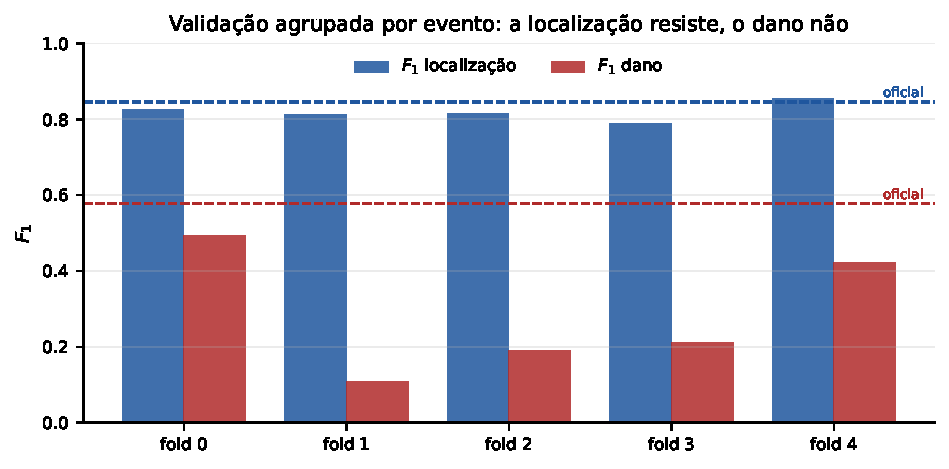
\includegraphics[width=0.86\linewidth]{figuras/folds.pdf}
\caption{Desempenho por \emph{fold} da validação agrupada por evento. As linhas
tracejadas marcam os valores do \emph{split} oficial. A localização (azul)
permanece próxima da referência em todos os \emph{folds}; o termo de dano
(vermelho) colapsa e varia fortemente conforme o evento excluído.}
\label{fig:folds}
\end{figure}

A interpretação é que a aparência do dano é específica do tipo de evento:
enchente, terremoto e furacão destroem de maneiras visualmente distintas, e um
modelo treinado em quatro tipos não extrapola para o quinto. A
Figura~\ref{fig:mapa} torna concreto o porquê: quando o \emph{fold} excluído
concentra incêndios florestais, por exemplo, o modelo precisa reconhecer
assinaturas de destruição --- estruturas reduzidas a fundações, ausência de
telhado, alteração cromática do terreno --- que os demais eventos não contêm.
Um sistema operacional de resposta a desastres calibrado pelo número oficial
estaria contando com uma capacidade que ele não possui.

\subsection{A mesma dissociação, por outro caminho}

A ablação que remove integralmente a imagem pós-desastre reproduz o padrão:

\begin{center}
\begin{tabular}{lrrr}
\toprule
& \textbf{$F_1$ loc.} & \textbf{$F_1$ dano} & \textbf{$F_1$ \texttt{destroyed}} \\
\midrule
Referência          & 0{,}8455 & 0{,}5781 & 0{,}731 \\
Sem ramo siamês     & 0{,}8416 & 0{,}3799 & 0{,}378 \\
\bottomrule
\end{tabular}
\end{center}

A localização não se altera ($-0{,}004$, dentro do ruído) e o termo de dano cai
34\%. Isso sustenta a hipótese central do desenho --- o sinal de dano provém da
comparação entre datas, não da aparência da cena --- mas registra que
$F_1^{\text{dano}} = 0{,}38$ ainda é obtido sem observar o pós-desastre, um piso
de vazamento contextual que merece investigação.

\subsection{Ablações}
\label{sec:ablacoes}

A Tabela~\ref{tab:ablacoes} reúne as quinze ablações, ordenadas por escore e
julgadas contra o piso de ruído da Seção~\ref{sec:desenho}.

\begin{table}[htbp]
\centering
\caption{Ablações de um fator, ordenadas por escore. Delta contra a referência
($0{,}6583$); veredito determinado pelo piso de ruído de $0{,}0068$.}
\label{tab:ablacoes}
\begin{tabular}{llrrl}
\toprule
\textbf{Fator alterado} & \textbf{Valor} & \textbf{Escore} & \textbf{$\Delta$} &
\textbf{Veredito} \\
\midrule
\emph{lr} do \emph{encoder} & $1{,}0\times$ (de $0{,}1\times$) & 0{,}6994 & $+0{,}0411$ & \textbf{melhor} \\
\emph{Encoder}              & \texttt{seresnext50}            & 0{,}6878 & $+0{,}0295$ & \textbf{melhor} \\
\emph{Encoder}              & \texttt{efficientnet\_b0}       & 0{,}6862 & $+0{,}0279$ & \textbf{melhor} \\
Perda de dano               & \texttt{ce\_dice} (sem focal)   & 0{,}6613 & $+0{,}0030$ & dentro do ruído \\
\multicolumn{2}{l}{\emph{(referência)}}                       & \emph{0{,}6583} & --- & --- \\
Fusão                       & \texttt{cat} (sem $|\Delta|$)   & 0{,}6563 & $-0{,}0020$ & dentro do ruído \\
Média móvel (EMA)           & $0{,}999$                       & 0{,}6516 & $-0{,}0067$ & dentro do ruído \\
Recorte                     & 768                             & 0{,}6495 & $-0{,}0088$ & pior \\
Reamostragem                & desligada                       & 0{,}6412 & $-0{,}0172$ & pior \\
Normalização                & ImageNet                        & 0{,}6382 & $-0{,}0202$ & pior \\
Cenas vazias                & excluídas                       & 0{,}6331 & $-0{,}0253$ & pior \\
Recorte                     & 256                             & 0{,}6248 & $-0{,}0335$ & pior \\
Fusão                       & \texttt{diff} (só $|\Delta|$)   & 0{,}6080 & $-0{,}0503$ & pior \\
Dados                       & sem \texttt{tier3}              & 0{,}5922 & $-0{,}0662$ & pior \\
Inicialização               & sem pré-treino                  & 0{,}5311 & $-0{,}1272$ & pior \\
Arquitetura                 & sem ramo siamês                 & 0{,}5184 & $-0{,}1399$ & pior \\
\bottomrule
\end{tabular}
\end{table}

\paragraph{Três resultados negativos limpos.}
A Equação~\ref{eq:fusao} assume que fornecer $|f^{\text{pós}}-f^{\text{pré}}|$
explicitamente beneficia o modelo. \textbf{Não beneficia}: removê-lo custa
$0{,}0020$, dentro do ruído --- a rede aprende a comparar por conta própria
quando recebe as duas representações concatenadas. O recíproco, contudo, não vale:
fornecer \emph{apenas} a diferença custa $0{,}0503$. Concatenar basta; subtrair
não basta. Trata-se da mesma dicotomia \emph{conc} versus \emph{diff} de Daudt
\emph{et al.}~\cite{daudt2018}, aqui resolvida a favor da concatenação.

Igualmente, a média móvel exponencial de pesos~\cite{tarvainen2017} não produziu
efeito mensurável, e o termo focal mostrou-se redundante quando pesos por classe
já estão aplicados: ambos os mecanismos atacam desbalanceamento, e usá-los em
conjunto não soma.

\paragraph{Capacidade não é o gargalo.}
Um \emph{encoder} com 6{,}19\,M de parâmetros empata com outro de 51{,}26\,M
($0{,}6862$ contra $0{,}6878$, diferença dentro do ruído), e ambos superam a
referência de 25{,}50\,M. Se capacidade limitasse o desempenho, o modelo maior
teria se distanciado do menor. A leitura correta não é ``mais parâmetros
ajudam'', e sim ``\texttt{resnet34} é a escolha inferior das três'' --- com a
consequência prática de que o problema pode ser tratado com um modelo 4$\times$
menor sem perda.

\paragraph{Curva de resolução.} Após a reavaliação em cena inteira, a curva é não
monotônica e o ótimo está no ponto intermediário: $0{,}6248$ (256), $0{,}6583$
(512) e $0{,}6495$ (768). Recortes menores perdem contexto; maiores reduzem o
número de amostras por passo no mesmo orçamento. A localização é insensível
(0{,}839--0{,}847): toda a variação reside no termo de dano.

\subsection{Dinâmica de treino}

A Figura~\ref{fig:curvas} acompanha quatro configurações ao longo das 20 épocas.
Três observações:

\begin{itemize}
  \item \textbf{A ablação sem pré-treino converge mais devagar e a um patamar
  inferior.} A curva de perda de treino permanece acima das demais durante toda
  a execução: não é questão de otimização mal ajustada, e sim de ponto de
  partida.

  \item \textbf{A ablação sem ramo siamês exibe perda de treino competitiva mas
  escore de validação estagnado} em torno de $0{,}52$. O modelo aprende a
  reduzir sua perda --- a localização é fácil --- sem que isso se converta em
  discriminação de severidade, exatamente o comportamento esperado de quem não
  observa o pós-desastre.

  \item \textbf{A ablação vencedora domina desde a época 5.} Liberar a taxa de
  aprendizado do \emph{encoder} não apenas eleva o patamar final: acelera toda a
  trajetória, o que reforça a leitura de que $0{,}1\times$ estava restringindo a
  adaptação ao domínio, e não regularizando.
\end{itemize}

\begin{figure}[htbp]
\centering
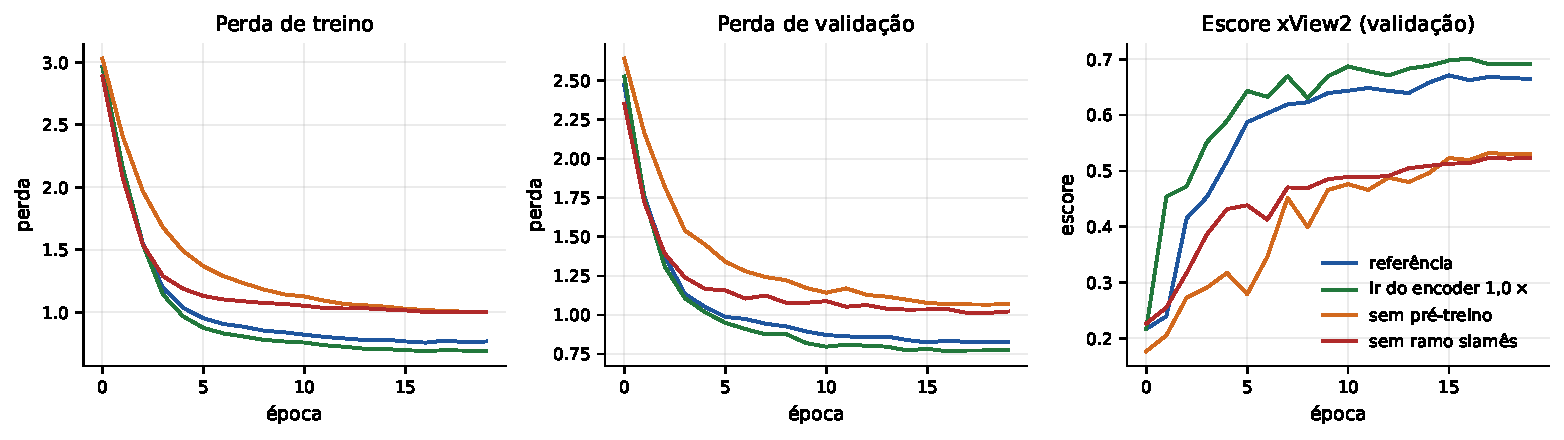
\includegraphics[width=\linewidth]{figuras/curvas.pdf}
\caption{Dinâmica de treino de quatro configurações. À esquerda e ao centro, as
perdas; à direita, o escore de validação por época. Note que perda de treino
baixa não implica escore alto: a variante sem ramo siamês minimiza a perda
razoavelmente bem e ainda assim estagna, porque o termo de localização --- fácil
--- domina a perda enquanto o de severidade domina a métrica.}
\label{fig:curvas}
\end{figure}

\subsection{Onde o modelo erra}
\label{sec:erros}

\begin{table}[htbp]
\centering
\caption{Desempenho por classe da configuração de referência.}
\label{tab:classes}
\begin{tabular}{lrrr}
\toprule
\textbf{Classe} & \textbf{$F_1$} & \textbf{Precisão} & \textbf{\emph{Recall}} \\
\midrule
\texttt{no-damage}    & 0{,}779 & 0{,}791 & 0{,}768 \\
\texttt{minor-damage} & \textbf{0{,}399} & \textbf{0{,}372} & \textbf{0{,}430} \\
\texttt{major-damage} & 0{,}567 & 0{,}514 & 0{,}633 \\
\texttt{destroyed}    & 0{,}731 & 0{,}739 & 0{,}724 \\
\bottomrule
\end{tabular}
\end{table}

Como a Equação~\ref{eq:metrica} emprega média harmônica, o escore é dominado pela
pior classe. A Tabela~\ref{tab:classes} identifica \texttt{minor-damage}, com
metade do $F_1$ de \texttt{no-damage}. \textbf{Melhorar essa classe isoladamente
vale mais do que melhorar as outras três em conjunto.}

O achado operacionalmente relevante é que o limitante é a \emph{precisão}
($0{,}372$) e não o \emph{recall} ($0{,}430$) --- padrão que se repete em 15 dos
18 experimentos com \emph{split} oficial, como mostra o painel direito da
Figura~\ref{fig:precrecall}. Isso \textbf{inverte a correção intuitiva}:
aumentar peso de classe e reamostragem elevaria o \emph{recall} às custas da
precisão, que já é o lado fraco. Note-se que, sem registrar precisão e
\emph{recall} separadamente, o diagnóstico seria impossível: $F_1$ e IoU são
funções um do outro ($F_1 = 2\,\mathrm{IoU}/(1+\mathrm{IoU})$) e, juntos, não
carregam essa informação.

\begin{figure}[htbp]
\centering
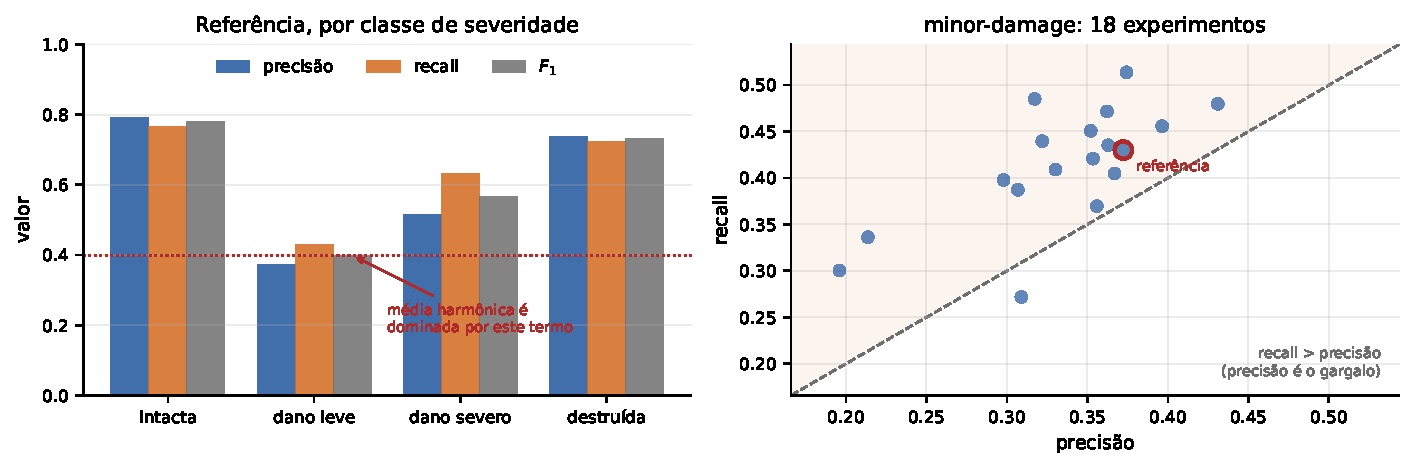
\includegraphics[width=\linewidth]{figuras/prec_recall.pdf}
\caption{Esquerda: desempenho por classe da referência; a linha pontilhada marca
o menor $F_1$, que determina a média harmônica. Direita: precisão contra
\emph{recall} da classe \texttt{minor-damage} nos 18 experimentos com
\emph{split} oficial. Praticamente todos caem acima da diagonal, isto é, com
\emph{recall} superior à precisão.}
\label{fig:precrecall}
\end{figure}

\begin{table}[htbp]
\centering
\caption{Matriz de confusão da referência, normalizada por linha (\% da classe
verdadeira). Avaliação em cena inteira sobre \texttt{hold}.}
\label{tab:confusao}
\begin{tabular}{lrrrrr}
\toprule
\textbf{Verdade $\backslash$ Predito} & \texttt{backgr.} & \texttt{no-dmg} &
\texttt{minor} & \texttt{major} & \texttt{destr.} \\
\midrule
\texttt{background}   & \textbf{99{,}0} & 0{,}7 & 0{,}1 & 0{,}1 & 0{,}1 \\
\texttt{no-damage}    & 14{,}5 & \textbf{76{,}8} & 5{,}7 & 2{,}9 & 0{,}2 \\
\texttt{minor-damage} & 16{,}9 & 23{,}0 & \textbf{43{,}0} & 16{,}4 & 0{,}6 \\
\texttt{major-damage} & 13{,}4 & 11{,}2 & 10{,}1 & \textbf{63{,}3} & 2{,}1 \\
\texttt{destroyed}    & 15{,}8 & 2{,}3 & 0{,}9 & 8{,}7 & \textbf{72{,}4} \\
\bottomrule
\end{tabular}
\end{table}

A Tabela~\ref{tab:confusao} e a Figura~\ref{fig:confusao} mostram que, dos
pixels verdadeiramente \texttt{minor-damage}, 23{,}0\% são classificados como
\texttt{no-damage} e 16{,}4\% como \texttt{major-damage}. A quase simetria entre
subestimar e superestimar sugere que a fronteira entre níveis é genuinamente
ambígua, e não um viés sistemático do modelo. Registre-se ainda que 13--17\% de
toda edificação danificada é perdida como fundo, em todas as classes de
severidade: um erro de localização que a métrica de dano contabiliza junto.

\begin{figure}[htbp]
\centering
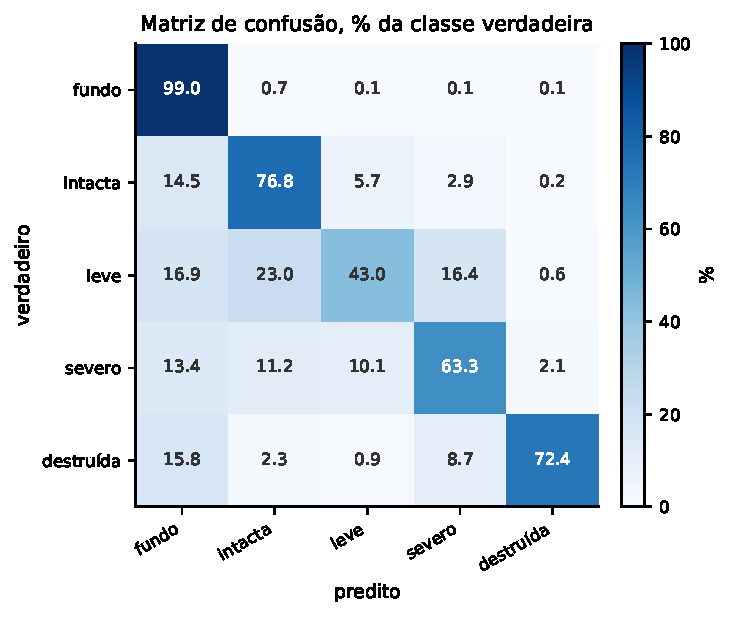
\includegraphics[width=0.62\linewidth]{figuras/confusao.pdf}
\caption{Matriz de confusão da configuração de referência, normalizada por linha.
A diagonal decresce de $99{,}0$ (fundo) a $43{,}0$ (\texttt{minor-damage}); a
massa fora da diagonal concentra-se nas células adjacentes, coerente com a
natureza ordinal dos rótulos.}
\label{fig:confusao}
\end{figure}

\subsection{Inspeção qualitativa}

A Figura~\ref{fig:exemplos} apresenta predições do melhor modelo em quatro cenas
de \texttt{hold}, escolhidas por composição de severidade no recorte avaliado.
As quatro linhas tornam visíveis os padrões que as tabelas quantificam:

\begin{itemize}
  \item \textbf{A delimitação das edificações é consistentemente precisa}, mesmo
  onde a classificação erra. Contornos, separação entre construções vizinhas e
  cobertura de estruturas pequenas correspondem bem à anotação. É o correlato
  visual de o $F_1$ de localização ser competitivo com o ranking oficial
  (Seção~\ref{sec:leaderboard}).

  \item \textbf{Os dois sentidos do erro de \texttt{minor-damage} aparecem lado a
  lado.} Na segunda linha, uma quadra majoritariamente intacta recebe marcações
  de dano leve --- falha de precisão. Na terceira, um galpão anotado como dano
  leve é classificado como intacto --- falha de \emph{recall}. As duas coexistem
  no mesmo modelo, o que é exatamente o que a quase simetria da
  Tabela~\ref{tab:confusao} prevê.

  \item \textbf{A severidade máxima é sistematicamente atenuada.} Na quarta
  linha, edificações anotadas como destruídas são preditas como dano severo. O
  erro é de um grau na escala ordinal, mas custa duas classes na média
  harmônica.
\end{itemize}

\begin{figure}[htbp]
\centering
\IfFileExists{figuras/exemplos.png}{%
  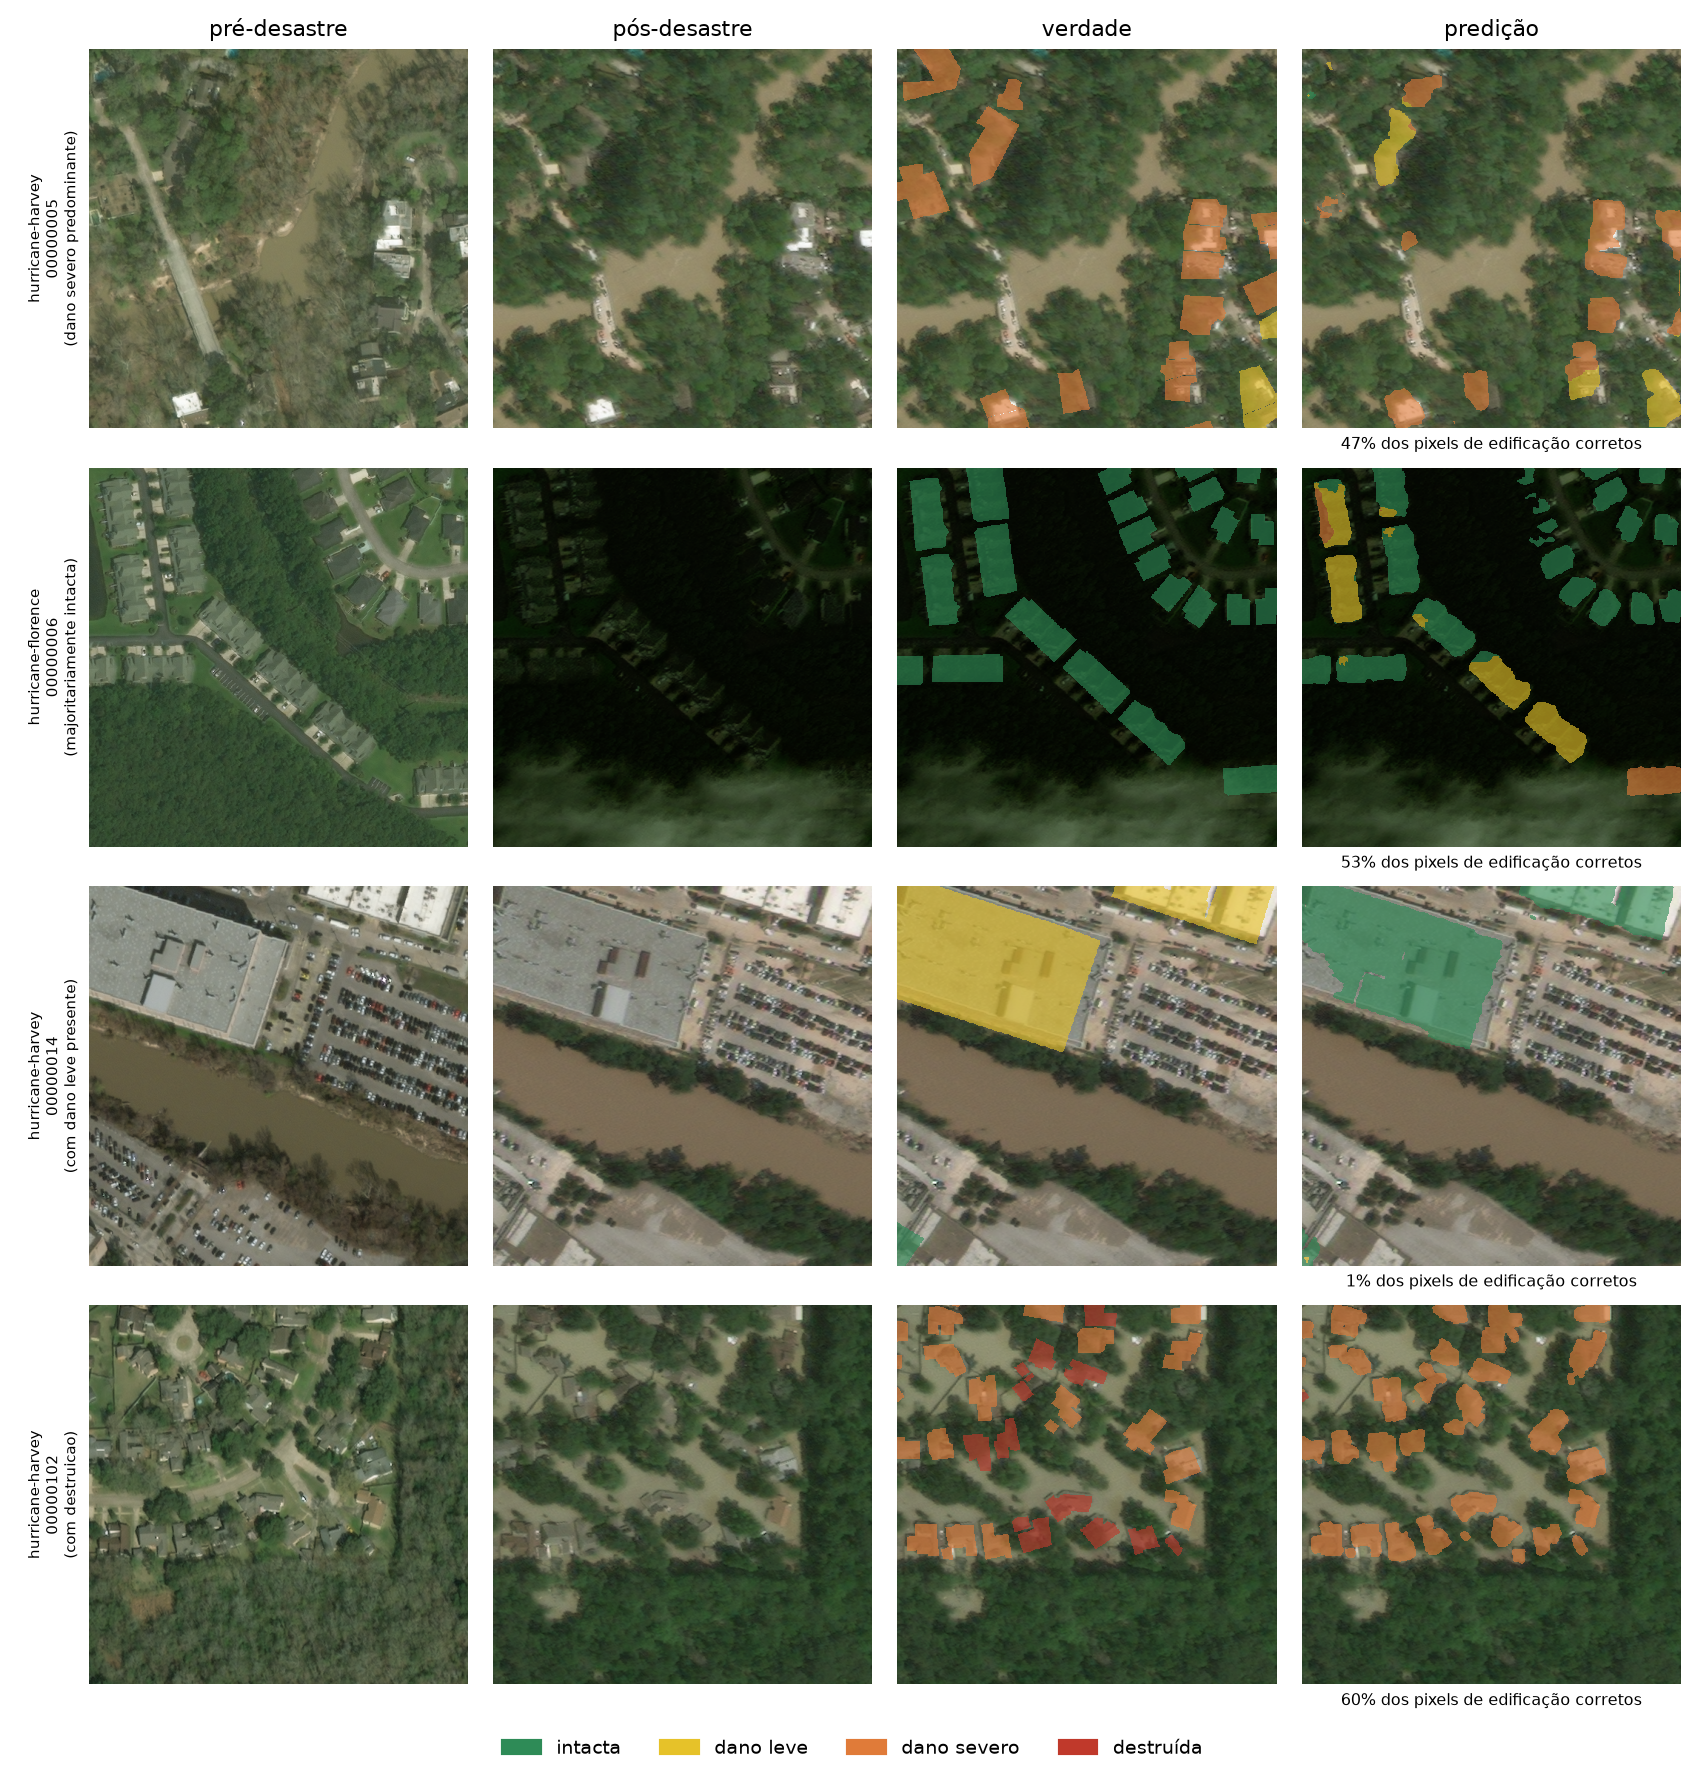
\includegraphics[width=\linewidth]{figuras/exemplos.png}%
}{%
  \fbox{\begin{minipage}[c][60mm][c]{0.96\linewidth}
    \centering\color{cinza}\small
    \textbf{[ exemplos qualitativos ]}\\[1mm]
    gere com \texttt{scripts/figuras\_pred.py}
  \end{minipage}}%
}
\caption{Predições do melhor modelo em quatro cenas de \texttt{hold}. Colunas:
imagem pré-desastre, pós-desastre, anotação de referência e predição. A fração
indicada sob cada predição é o percentual de pixels de edificação classificados
corretamente naquele recorte.}
\label{fig:exemplos}
\end{figure}

\section{Comparação com o ranking oficial}
\label{sec:leaderboard}

O desafio xView2 publica uma tabela de classificação com o desempenho das
submissões avaliadas em sua partição reservada (Figura~\ref{fig:lbprint}).
Confrontar nosso melhor modelo com ela situa o trabalho, desde que as ressalvas
abaixo sejam observadas.

\begin{figure}[htbp]
\centering
\IfFileExists{figuras/leaderboard.png}{%
  \includegraphics[width=\linewidth]{figuras/leaderboard.png}%
}{%
  \fbox{\begin{minipage}[c][38mm][c]{0.96\linewidth}
    \centering\color{cinza}\small
    \textbf{[ captura da tabela de classificação do xView2 ]}\\[1mm]
    salve como \texttt{figuras/leaderboard.png}
  \end{minipage}}%
}
\caption{Nove primeiras colocações do ranking oficial do xView2, com o escore
global e a decomposição por classe. Fonte: plataforma do
desafio~\cite{xview2}.}
\label{fig:lbprint}
\end{figure}

\subsection{Ressalvas de comparabilidade}

\begin{enumerate}
  \item \textbf{Partições distintas.} O ranking avalia a partição reservada do
  desafio; nós avaliamos \texttt{hold}.

  \item \textbf{Viés de seleção a nosso favor.} O \emph{checkpoint} reportado é o
  de melhor escore \emph{nessa mesma partição} \texttt{hold}, usada também para
  seleção de modelo. Nosso número é, portanto, otimista --- e ainda assim
  inferior.

  \item \textbf{Orçamento incomparável.} Reportamos um único modelo treinado por
  20 épocas, sem \emph{ensemble}, sem aumento em tempo de teste e sem busca de
  hiperparâmetros. As submissões do topo empregam rotineiramente os três.
\end{enumerate}

A conclusão correta é que a diferença medida é um \emph{piso}: o modelo real
ficaria abaixo do que a Tabela~\ref{tab:leaderboard} indica, e não acima.

\subsection{Resultado}

\begin{table}[htbp]
\centering
\caption{Melhor modelo deste trabalho contra a faixa das nove primeiras
colocações oficiais. Valores em $F_1$.}
\label{tab:leaderboard}
\begin{tabular}{lrrrl}
\toprule
\textbf{Métrica} & \textbf{1\textordmasculine} & \textbf{9\textordmasculine} &
\textbf{Este trabalho} & \textbf{Situação} \\
\midrule
$F_1$ global            & 0{,}81193 & 0{,}73289 & 0{,}69942 & abaixo do 9\textordmasculine \\
$F_1$ localização       & 0{,}86350 & 0{,}85250 & \textbf{0{,}85562} & \textbf{dentro da faixa (6\textordmasculine)} \\
\texttt{no-damage}      & 0{,}92344 & 0{,}88864 & 0{,}80816 & abaixo do 9\textordmasculine \\
\texttt{minor-damage}   & 0{,}64445 & 0{,}47583 & 0{,}45407 & abaixo do 9\textordmasculine \\
\texttt{major-damage}   & 0{,}78591 & 0{,}71313 & 0{,}64962 & abaixo do 9\textordmasculine \\
\texttt{destroyed}      & 0{,}86403 & 0{,}80700 & 0{,}74332 & abaixo do 9\textordmasculine \\
\bottomrule
\end{tabular}
\end{table}

\begin{figure}[htbp]
\centering
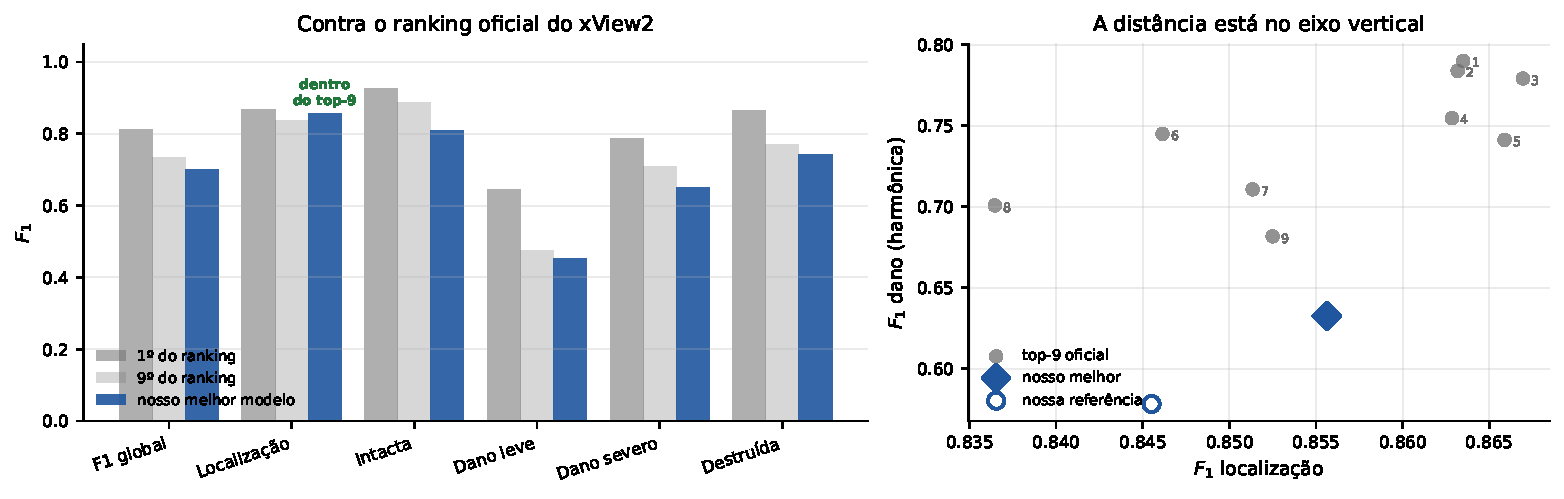
\includegraphics[width=\linewidth]{figuras/leaderboard.pdf}
\caption{Esquerda: comparação por métrica contra o primeiro e o nono colocados.
Direita: o mesmo dado projetado no plano localização $\times$ dano; os números
identificam a colocação oficial. A distância até o grupo do topo é quase
inteiramente vertical.}
\label{fig:leaderboard}
\end{figure}

O resultado é acentuadamente assimétrico, e reproduz --- por um terceiro caminho
independente --- o achado central deste trabalho. Em \textbf{localização}, o
valor de $0{,}85562$ situa-se dentro da faixa das nove primeiras colocações
($0{,}83646$ a $0{,}86695$), o que corresponderia à sexta posição. Em todas as
quatro classes de severidade, o modelo fica abaixo da nona colocação.

O painel direito da Figura~\ref{fig:leaderboard} explicita a geometria: no eixo
horizontal, nosso modelo está no meio do grupo de topo; no vertical, separado
por uma lacuna de aproximadamente $0{,}05$ a $0{,}16$ na média harmônica das
severidades. \textbf{A diferença para o estado da arte não está em encontrar
edificações --- está em graduar o dano.}

Isso posiciona o esforço subsequente com precisão. Ganhos em segmentação
(arquitetura de \emph{decoder}, resolução, pós-processamento de contornos)
atacariam a dimensão em que já somos competitivos. O retorno está na dimensão
ortogonal, e a Seção~\ref{sec:erros} indica onde especificamente: a precisão de
\texttt{minor-damage}, que é também a classe de maior lacuna absoluta contra o
ranking ($0{,}454$ contra $0{,}644$ do primeiro colocado).

\section{Limitações}

\begin{itemize}
  \item \textbf{Orçamento de 20 épocas.} O escore médio máximo ocorreu na época
  16{,}8 de 19, e apenas 9 dos 18 experimentos atingiram o pico na última época.
  Os valores absolutos ficam abaixo do que estas arquiteturas alcançam; as
  \emph{comparações} permanecem válidas, pois todos receberam idêntico orçamento.

  \item \textbf{Uma semente por ablação.} O piso de ruído foi medido apenas na
  configuração de referência e extrapolado às demais. Deltas de $+0{,}03$ a
  $+0{,}04$ representam 4--6$\times$ esse piso e são provavelmente reais; deltas
  de $\pm0{,}01$ a $\pm0{,}02$ mereceriam réplica antes de sustentar afirmação.

  \item \textbf{Co-registro assumido.} O dataset replica os polígonos do pré no
  pós, assumindo alinhamento perfeito entre as datas. Desalinhamento real
  converte-se em ruído de rótulo silencioso, que nenhum experimento aqui mede.

  \item \textbf{Ausência de conjunto de teste intocado.} A partição
  \texttt{hold} serve simultaneamente de validação e de número reportado; a
  partição \texttt{test} do xBD permanece sem uso.

  \item \textbf{Heterogeneidade de \texttt{tier3}.} A qualidade de anotação de
  \texttt{tier3} difere de \texttt{tier1}, e o estudo os trata como
  equivalentes; a ablação correspondente mede o efeito agregado, não a diferença
  de qualidade.
\end{itemize}

\section{Conclusão}

Executamos um estudo de ablação de 24 configurações sobre o xBD em um único dia
de laboratório, coordenando 10 estações por uma fila com posse exclusiva. O
resultado principal é que o protocolo oficial do xView2 superestima em 32{,}3\% a
generalização, e que essa superestimação é quase inteiramente atribuível ao termo
de severidade: localizar edificações transfere para um desastre novo, graduar
danos não transfere.

Do lado metodológico, três componentes usualmente assumidos como benéficos ---
a diferença explícita em espaço de \emph{features}, a média móvel de pesos e o
termo focal --- não produziram efeito acima do ruído, e podem ser removidos sem
custo. Capacidade de modelo não se mostrou limitante. O maior ganho isolado
($+0{,}0411$) veio de não frear a taxa de aprendizado do \emph{encoder}
pré-treinado, prática herdada de regimes de ajuste fino longo e inadequada ao
orçamento aqui empregado.

Finalmente, o diagnóstico por classe indica que o esforço subsequente deve ser
dirigido à \emph{precisão} da classe \texttt{minor-damage} --- e não ao seu
\emph{recall}, para o qual apontariam as correções convencionais de
desbalanceamento.

\section*{Disponibilidade}

Código, matriz de experimentos, documentação metodológica e resultados
reavaliados estão disponíveis em
\url{https://github.com/Tulio-CS/Disaster-Damage}. Os pesos dos 24 modelos
($\approx$10\,GB) estão disponíveis mediante solicitação.

% =====================================================================
\begin{thebibliography}{99}
\small

\bibitem{gupta2019}
R.~Gupta \emph{et al.},
\newblock ``Creating xBD: A Dataset for Assessing Building Damage from Satellite
Imagery,''
\newblock \emph{CVPR Workshops}, 2019. arXiv:1911.09296.

\bibitem{xview2}
\newblock \emph{xView2 Challenge}. \url{https://xview2.org}.
\newblock Define a métrica oficial e as partições do dataset.

\bibitem{xview2solutions}
\newblock Soluções vencedoras do xView2, \url{https://github.com/DIUx-xView}.

\bibitem{daudt2018}
R.~C. Daudt, B.~Le~Saux, A.~Boulch,
\newblock ``Fully Convolutional Siamese Networks for Change Detection,''
\newblock \emph{IEEE ICIP}, 2018. arXiv:1810.08462.

\bibitem{bromley1993}
J.~Bromley \emph{et al.},
\newblock ``Signature Verification using a `Siamese' Time Delay Neural
Network,''
\newblock \emph{NIPS}, 1993.

\bibitem{ronneberger2015}
O.~Ronneberger, P.~Fischer, T.~Brox,
\newblock ``U-Net: Convolutional Networks for Biomedical Image Segmentation,''
\newblock \emph{MICCAI}, 2015. arXiv:1505.04597.

\bibitem{he2016}
K.~He \emph{et al.},
\newblock ``Deep Residual Learning for Image Recognition,''
\newblock \emph{CVPR}, 2016. arXiv:1512.03385.

\bibitem{xie2017}
S.~Xie \emph{et al.},
\newblock ``Aggregated Residual Transformations for Deep Neural Networks,''
\newblock \emph{CVPR}, 2017. arXiv:1611.05431.

\bibitem{hu2018}
J.~Hu, L.~Shen, G.~Sun,
\newblock ``Squeeze-and-Excitation Networks,''
\newblock \emph{CVPR}, 2018. arXiv:1709.01507.

\bibitem{tan2019}
M.~Tan, Q.~Le,
\newblock ``EfficientNet: Rethinking Model Scaling for Convolutional Neural
Networks,''
\newblock \emph{ICML}, 2019. arXiv:1905.11946.

\bibitem{timm}
R.~Wightman,
\newblock \emph{PyTorch Image Models} (\texttt{timm}),
\newblock \url{https://github.com/huggingface/pytorch-image-models}.

\bibitem{lin2017focal}
T.-Y. Lin \emph{et al.},
\newblock ``Focal Loss for Dense Object Detection,''
\newblock \emph{ICCV}, 2017. arXiv:1708.02002.

\bibitem{milletari2016}
F.~Milletari, N.~Navab, S.-A. Ahmadi,
\newblock ``V-Net: Fully Convolutional Neural Networks for Volumetric Medical
Image Segmentation,''
\newblock \emph{3DV}, 2016. arXiv:1606.04797.

\bibitem{lin2014coco}
T.-Y. Lin \emph{et al.},
\newblock ``Microsoft COCO: Common Objects in Context,''
\newblock \emph{ECCV}, 2014. arXiv:1405.0312.

\bibitem{loshchilov2019}
I.~Loshchilov, F.~Hutter,
\newblock ``Decoupled Weight Decay Regularization,''
\newblock \emph{ICLR}, 2019. arXiv:1711.05101.

\bibitem{loshchilov2017}
I.~Loshchilov, F.~Hutter,
\newblock ``SGDR: Stochastic Gradient Descent with Warm Restarts,''
\newblock \emph{ICLR}, 2017. arXiv:1608.03983.

\bibitem{micikevicius2018}
P.~Micikevicius \emph{et al.},
\newblock ``Mixed Precision Training,''
\newblock \emph{ICLR}, 2018. arXiv:1710.03740.

\bibitem{tarvainen2017}
A.~Tarvainen, H.~Valpola,
\newblock ``Mean teachers are better role models,''
\newblock \emph{NeurIPS}, 2017. arXiv:1703.01780.

\bibitem{roberts2017}
D.~R. Roberts \emph{et al.},
\newblock ``Cross-validation strategies for data with temporal, spatial,
hierarchical, or phylogenetic structure,''
\newblock \emph{Ecography}, vol.~40, n.~8, pp.~913--929, 2017.

\end{thebibliography}

\end{document}
